\section{Dealing with imbalanced data}

\subsection{Motivation}

\begin{frame}\frametitle{\subsecname}

\only<1>{
Proportion of class labels in the dataset is not uniform.
Not the same as ``easy vs. difficult'' classes. This is only about class frequency.
}

\slidesonly{\vspace{-5mm}}

\begin{figure}[ht]
     \centering
     \savebox{\imagebox}{
	 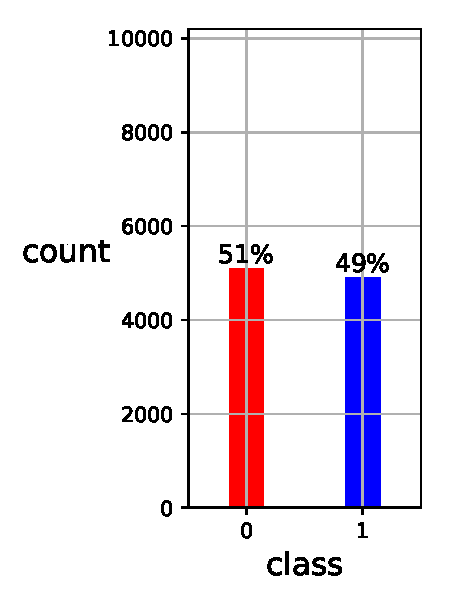
\includegraphics[width=0.28\textwidth]{img/hist_balanced}}%
     \begin{subfigure}[t]{0.28\textwidth}
         \centering
         \usebox{\imagebox}% Place largest image
         \caption{balanced $\approx 1:1$}
     \end{subfigure}
     \hspace{5mm}
     \begin{subfigure}[t]{0.28\textwidth}
         \centering
         \raisebox{\dimexpr.5\ht\imagebox-.5\height}{% Raise smaller image into place
         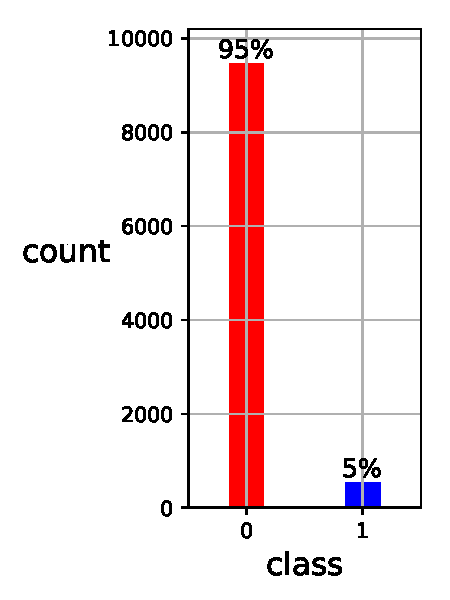
\includegraphics[width=0.99\textwidth]{img/hist_imbalanced}
         }
         \caption{highly unbalanced}
         \label{fig:linear}
     \end{subfigure}
\end{figure} 

\only<2>{     
A strong imbalance leads to the classifier learning a trivial solution that indeed minimizes the average cost over the training samples.
}
\only<2>{
\begin{equation}
E^T = \frac{1}{p} \sum_{\alpha=1}^p e^{(\alpha)}
\end{equation}
}
\only<3>{
\begin{equation}
E^T = \frac{1}{p} \Big\lbrack
{\color{blue}\sum_{\beta\,\in D_{+}}^{|D_{+}|} e^{(\beta)}}
+
{\color{red}\sum_{\beta\,\in D_{-}}^{|D_{-}|} e^{(\beta)}}
\Big\rbrack
\end{equation}

\mode<article>{
where set $D_{+}$ and $D_{-}$ are the subsets of data of only positive and negative samples, respectively:

\begin{equation}
{
\color{blue}
D_{+} := 
\Big\{ \left(\vec x^{(\alpha)}, \vec y^{(\alpha)}_{T} \right) \Big|\,y^{(\alpha)}_{T} > 0 \,\Big\}
\quad \text{(subset of positive samples)}
}
\end{equation}

and 

\begin{equation}
{
\color{red}
D_{-} := 
\Big\{ \left(\vec x^{(\alpha)}, \vec y^{(\alpha)}_{T} \right) \Big|\,y^{(\alpha)}_{T} \le 0 \,\Big\}
\quad \text{(subset of positive samples)}
}
\end{equation}

}

By always predicting ``0'' it will be correct 95\% of the time.
}
\end{frame}

\subsection{Confusion matrix}

\begin{frame}\frametitle{\subsecname}

The confusion matrix differentiates between the types of mistakes a classifier makes.

\begin{tabular}{ll|l|l|l}
\cline{3-4}
												  &          & \multicolumn{2}{c|}{Ground truth label}                        &  \\ \cline{3-4}
												  &          & \multicolumn{1}{c|}{Positive} & \multicolumn{1}{c|}{Negative}  &  \\ \cline{3-4}
												  &          & \multicolumn{1}{c|}{``Cat''} & \multicolumn{1}{c|}{``not Cat''}  &  \\ \cline{1-4}
\multicolumn{1}{|r|}{\multirow{2}{*}{Prediction}} & Positive & \textbf{T}rue \textbf{P}ositives & \textbf{F}alse \textbf{P}ositives &  \\ \cline{2-4}
\multicolumn{1}{|r|}{}                            & Negative &  \textbf{F}alse \textbf{N}egatives & \textbf{T}rue \textbf{N}egatives &  \\ \cline{1-4}
												  &          & \multicolumn{1}{c|}{$P$} & \multicolumn{1}{c|}{$N$}  &  \\ \cline{3-4}
\end{tabular}	


\end{frame}

\subsection{Performance metrics}

\begin{frame}\frametitle{\subsecname}

\mode<presentation>{
\begin{tabular}{ll|l|l|l}
\cline{3-4}
												  &          & \multicolumn{2}{c|}{Ground truth label}                        &  \\ \cline{3-4}
												  &          & \multicolumn{1}{c|}{Positive} & \multicolumn{1}{c|}{Negative}  &  \\ \cline{3-4}
												  &          & \multicolumn{1}{c|}{``Cat''} & \multicolumn{1}{c|}{``not Cat''}  &  \\ \cline{1-4}
\multicolumn{1}{|r|}{\multirow{2}{*}{Prediction}} & Positive & \textbf{T}rue \textbf{P}ositives & \textbf{F}alse \textbf{P}ositives &  \\ \cline{2-4}
\multicolumn{1}{|r|}{}                            & Negative &  \textbf{F}alse \textbf{N}egatives & \textbf{T}rue \textbf{N}egatives &  \\ \cline{1-4}
												  &          & \multicolumn{1}{c|}{$P$} & \multicolumn{1}{c|}{$N$}  &  \\ \cline{3-4}
\end{tabular}	

}

\begin{equation}
 \text{ fraction of correct classifications } 
 \corresponds \text{ Accuracy }
 = \frac{T\kern-.4ex P+T\kern-.4exN}{P+N}
\end{equation}

\only<2>{
\slidesonly{
{\placeimage{12.5}{10.}{img/hist_imbalanced}{width=25mm}}
}

In our imbalanced example:
\begin{equation}
\frac{T\kern-.4exP+T\kern-.5exN}{P+N} = \frac{0+9500}{500+9500} = 0.95
\end{equation}

\notesonly{
Accuracy is a misleading metric when the classes are imbalanced.
}
}

\only<3>{
Other metrics:

How many of the positive labels did we get:

\begin{equation}
\text{sensitivity (recall) }
 = \frac{T\kern-.4exP}{P}
\end{equation}

\mode<article>{
and how often were we correct, whenever we predicted positive?

\begin{equation}
\text{precision }
 = \frac{T\kern-.4exP}{T\kern-.4exP+F\kern-.5exP}
\end{equation}

Recall and precision can be combined into:

\begin{equation}
\text{F1 score }
 = 2 \cdot \frac{\mathrm{recall} \times \mathrm{precision}}{\mathrm{recall} + \mathrm{precision}}
\end{equation}
}

Similarly, for the negative class. How many of the negative class did we get:

\begin{equation}
\text{specificity}
 = \frac{T\kern-.5exN}{N}
\end{equation}

\mode<article>{
Recall and specificity can be combined into:


\begin{equation}
\text{Balanced Accuracy }
 = \frac{1}{2} (\mathrm{recall} + \mathrm{specificity})
\end{equation}

``F1 score'' and ``Balanced Accuracy'' are common choices for assessing performance of a classifier evaluated on imbalanced data with different implications with regards to how ``consistent'' this imbalance is. 

}
}

\end{frame}




